\chapter{Conclusions and open questions}

\section{Synthesis of the programme}

The completed studies support a simple organizing statement: the B-stack waveform is
low-dimensional, but the value of machine learning depends on where the independent
information enters the problem.  When the target is an independent waveform-shape
closure, machine-learning methods often win decisively.  When the leading effect is
already described by an analytic detector model, the best traditional method is
competitive or superior.  When the label is derived from the same waveform quantity
used as an input, apparent machine-learning gains are not accepted as physics
measurements.

All quantitative conclusions in this chapter inherit the programme's reproduce-first
discipline.  The standard B-stave selection is formed directly from raw \texttt{HRDv}
waveforms,
\[
  b_i = {\rm median}(x_{i,0},x_{i,1},x_{i,2},x_{i,3}), \qquad
  A_i = \max_s (x_{i,s}-b_i),
\]
with selected pulses satisfying \(A_i>1000\) ADC on the B2, B4, B6, or B8 even
readout.  The raw selected-pulse count reproduced throughout the programme is
\(640737\).  Timing summaries use the robust central width
\[
  \sigma_{68} = \frac{Q_{0.84}(r)-Q_{0.16}(r)}{2},
\]
where \(r\) is the corrected timing residual.  Amplitude and energy closures use
\[
  {\rm res}_{68}=Q_{0.68}\left(\left|\frac{\widehat{y}-y}{y}\right|\right),
\]
and all quoted confidence intervals are bootstrap intervals, usually with runs or
held-out run blocks resampled as the correlation unit.

\section{What is understood}

\subsection{Timing is mostly analytic timewalk, not a deep-network problem}

The first timing result showed that a Ridge residual corrector on CFD20 improved a
global template-phase pickoff on held-out run 65, reducing pairwise \(\sigma_{68}\)
from \(2.889\) ns to \(1.846\) ns.  The follow-up analytic study changed the
interpretation: an explicit amplitude timewalk model reached \(1.495\) ns, while a
Ridge correction on template phase reached \(1.392\) ns.  Thus the large initial
gain was not evidence that a neural timing model had discovered a hidden degree of
freedom; most of it was an interpretable amplitude-dependent timewalk correction.
Waveform MLP and CNN studies later confirmed the pattern: learned waveform timing can
be useful as a residual diagnostic, but it does not replace the strongest analytic
timewalk baseline.

\begin{figure}[H]
  \centering
  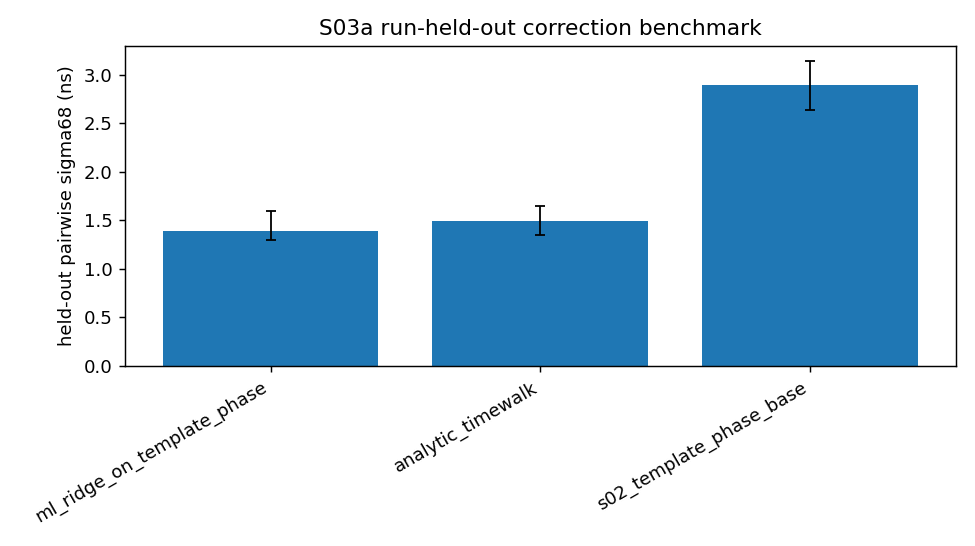
\includegraphics[width=0.78\linewidth]{../figures/reports/1781000705.514827.50025402__s03a_analytic_timewalk_correction/fig_s03a_head_to_head.png}
  \caption{Timing head-to-head from the analytic timewalk closure.  The initial ML gain over a global template is largely closed by an explicit amplitude model.}
\end{figure}

\subsection{The pile-up headline is limited by live-time, not by classifier score}

The most important rate-level revision is that the original \(R_{\max}\) estimate
used \(\tau_{\rm eff}=90\) ns as an assumption.  Direct waveform live-time estimates
do not recover that value.  At the 10\% tail crossing, the traditional template
estimate gives \(124.79\) ns with CI \([123.32,126.33]\) ns, implying a rescaled
combined \(R_{\max}\) near \(3.05\) MHz rather than \(4.22\) MHz.  Scanning the tail
threshold changes the numerical live-time but does not restore a 90 ns measured
window.

For two-pulse recovery, compact MLP/CNN methods can resolve shorter synthetic
separations and reduce timing RMS, but they also raise failure rates.  A representative
template-like injection benchmark found a bounded two-pulse fit live-time of 60 ns
with time RMS \(13.83\) ns and failure rate 0.172, while the compact ML method reached
20 ns with time RMS \(9.41\) ns but failure rate 0.323.  That is a method-ranking
result for controlled injections, not a final real-pile-up measurement.

\begin{figure}[H]
  \centering
  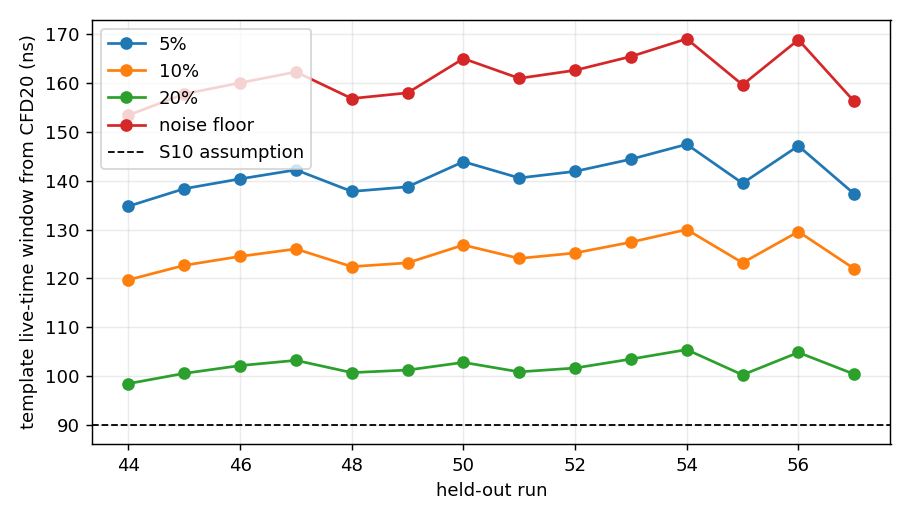
\includegraphics[width=0.82\linewidth]{../figures/reports/1781007337.1308.7dc86005/fig_threshold_scan_by_run.png}
  \caption{Threshold-scan live-time summary.  All tested waveform definitions remain above the 90 ns assumption used by the original rate estimate.}
\end{figure}

\subsection{Pulse shape is compact, and ML wins only in the compact regime}

The pulse-shape representation studies found that the first three PCA components
capture about 89\% of shape variance and eight components capture about 99.7\%.
A small autoencoder beats PCA by 40--51\% in reconstruction MSE for two to four
latent dimensions, but PCA wins at eight dimensions.  The conclusion is not that
the pulse is intrinsically high-dimensional; it is that a compact nonlinear embedding
is a useful summary when downstream tasks need only a few coordinates.

The same line of work is also the programme's clearest leakage lesson.  Learned
representations repeatedly failed to produce robust downstream superiority once
run-family and event-block shuffle controls were applied.  Conversely, shape-only ML
does win on injected corruption labels where the truth is independent of the input
definition.  The distinction is central: ML wins are accepted only when the target is
not a disguised restatement of the feature construction.

\subsection{Shape-dependent amplitude closures are the strongest ML wins}

The largest accepted ML gains are in waveform-shape closures with independent targets.
On duplicate odd-readout amplitude and charge, hist-gradient-boosted trees reduced
held-out amplitude res68 from 0.1238 for calibrated peak amplitude to 0.0091, and
charge res68 from 0.1954 for calibrated integral charge to 0.0151.  On artificial
constant-ceiling saturation, gradient boosting recovered true amplitude at roughly
3--5\% res68, compared with 10--29\% for a fixed-template rising-edge extrapolation.
These are real wins, but their domain is explicit: duplicate-readout and simulated
saturation closure, not absolute per-event beam energy without a truth bridge.

\begin{figure}[H]
  \centering
  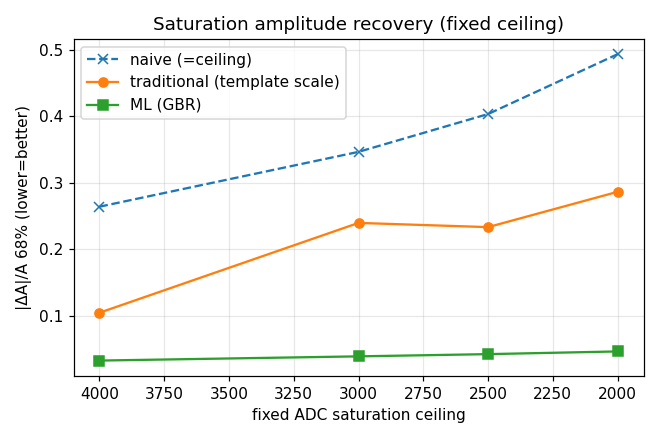
\includegraphics[width=0.78\linewidth]{../figures/reports/P07_saturation_recovery/fig_saturation_recovery.png}
  \caption{Saturation recovery on constant-ceiling artificial clips.  The leakage-fixed gradient-boosted regressor degrades more slowly than the fixed-template extrapolation as clipping becomes more severe.}
\end{figure}

\subsection{Pedestal studies identify a pathology, not a final correction}

The adaptive positivity-constrained pedestal is not validated by its zero-violation
construction.  Against leave-one-pretrigger-out targets on held-out runs 57 and 65,
it has MAE \(341.04\) ADC and mean bias \(-310.69\) ADC; the simple mean/median
baselines are better, and a calibrated HGB regressor reaches MAE \(48.88\) ADC.  The
ML result is useful as a contamination diagnostic, but the current mirror contains no
true forced/random pedestal sample.  The honest conclusion is therefore that large
adaptive lowering tags waveform contamination or pathology until a zero-signal
validation source is found.

\begin{figure}[H]
  \centering
  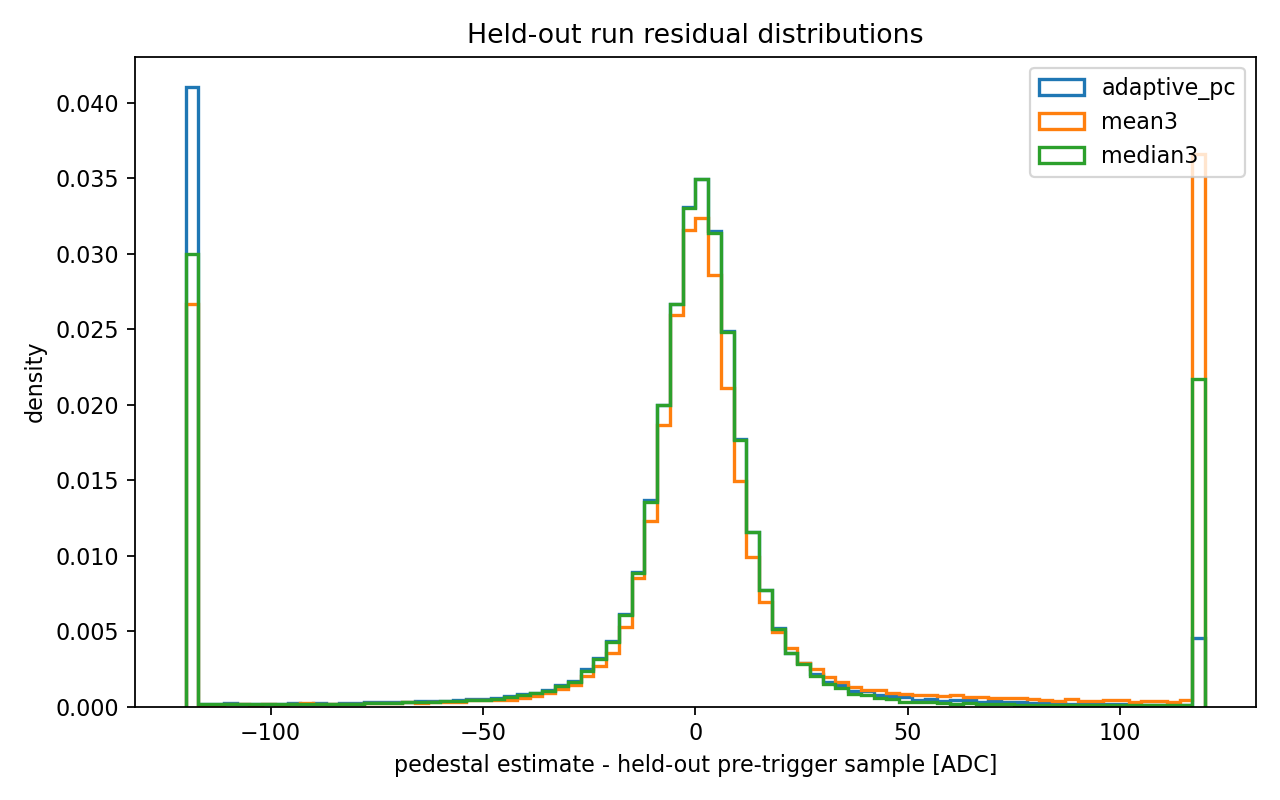
\includegraphics[width=0.78\linewidth]{../figures/reports/1780997954.15337.77205a71__s16_pedestal_baseline_validation/fig_heldout_residual_distributions.png}
  \caption{Held-out pedestal residual distributions.  The adaptive positivity constraint is biased on an independent pretrigger-sample benchmark.}
\end{figure}

\section{Representative numerical verdicts}

\begin{table}[H]
  \centering
  \footnotesize
  \setlength{\tabcolsep}{3pt}
  \begin{tabular}{@{}>{\raggedright\arraybackslash}p{0.12\linewidth}>{\raggedright\arraybackslash}p{0.16\linewidth}>{\raggedright\arraybackslash}p{0.11\linewidth}>{\raggedright\arraybackslash}p{0.34\linewidth}>{\raggedright\arraybackslash}p{0.11\linewidth}@{}}
    \toprule
    Topic & Strong traditional method & ML/NN method & Primary result & Verdict \\
    \midrule
    Timing pickoff & template phase & Ridge on CFD20 & \(2.889\,[2.639,3.205]\) ns vs \(1.846\,[1.521,2.014]\) ns & ML wins initial scan \\
    Analytic timewalk & amplitude timewalk & Ridge residual & \(1.495\,[1.347,1.644]\) ns vs \(1.392\,[1.297,1.596]\) ns & analytic closes most gain \\
    Live-time & template tail & Ridge live-time & \(124.79\,[123.32,126.33]\) ns vs \(123.22\,[120.71,125.61]\) ns & no 90 ns recovery \\
    Two-pulse closure & bounded template fit & compact MLP & 60 ns \([40,60]\), fail 0.172 vs 20 ns \([15,60]\), fail 0.323 & ML RMS win, adoption gated \\
    Duplicate amplitude & calibrated peak & HGB & res68 \(0.1238\,[0.1221,0.1251]\) vs \(0.0091\,[0.0090,0.0093]\) & ML wins \\
    Duplicate charge & calibrated integral & HGB & res68 \(0.1954\,[0.1936,0.1975]\) vs \(0.0151\,[0.0148,0.0153]\) & ML wins \\
    Saturation & rising-edge template & GBR & res68 0.104--0.286 vs 0.032--0.046 & ML wins on clips \\
    Pedestal proxy & mean3 / median3 & calibrated HGBR & MAE \(260.70\,[236.25,287.99]\) vs \(48.88\,[43.82,55.29]\) ADC & ML diagnostic win \\
    \bottomrule
  \end{tabular}
  \caption{Representative head-to-head results.  Bracketed intervals are bootstrap 95\% CIs when reported by the source study.}
\end{table}

\section{GEANT4 and the truth boundary}

The data-only programme has a hard boundary: absolute energy and particle identity
cannot be proven from HRD waveform data alone.  GEANT4 is therefore not an optional
polish step; it is the required truth bridge for deciding whether charge/depth
patterns correspond to proton/deuteron identity and deposited energy.  The first
schema audit showed that the external \texttt{hibeam\_g4} code can be built and can
write a truth tree in a patched smoke run, but the exact supplied production macro was
blocked by an unregistered \texttt{/ElGen/CSFile} command.  That result is valuable
because it turns ``GEANT4 needed'' into a concrete software-interface problem rather
than a vague future task.

A later truth-anchored energy calibration used a high-statistics GEANT4 truth tree as
a layer-level prior rather than an event-aligned truth match.  That model panel is
important because it tested the exact class of methods that might be proposed for a
final energy regressor: ridge, gradient-boosted trees, a tabular MLP, a 1D-CNN, and a
new physics-residual MLP architecture.  The winner was not a neural network.  The
GEANT4 Birks lookup, a traditional truth-anchored calibration, achieved the best
held-out res68.

\begin{table}[H]
  \centering
  \scriptsize
  \begin{tabular}{llll}
    \toprule
    Method & Family & Held-out res68 & Bootstrap 95\% CI \\
    \midrule
    GEANT4 Birks lookup & traditional truth-anchored & 0.04024 & [0.03886, 0.04161] \\
    Gradient-boosted trees & ML tree & 0.05669 & [0.04880, 0.06720] \\
    Physics-residual MLP & new neural residual & 0.05868 & [0.04902, 0.07788] \\
    Ridge & ML linear & 0.09667 & [0.08872, 0.11721] \\
    1D-CNN & neural waveform & 0.26570 & [0.24927, 0.28908] \\
    Old power law & traditional empirical & 0.46236 & [0.44431, 0.56438] \\
    Tabular MLP & neural tabular & 0.69235 & [0.68424, 0.69965] \\
    \bottomrule
  \end{tabular}
  \caption{Truth-anchored energy model panel.  The winner is the traditional GEANT4 Birks lookup; learned methods do not supersede the physics prior in this benchmark.}
\end{table}

\section{Systematics and caveats}

Several systematic limits recur across the programme.  First, run splitting is
necessary but not sufficient.  Some labels, especially \(D_t\), curvature, and
downstream tail definitions, are partly functions of the same waveform features used
by the model.  A classifier can score near perfectly in that setting without
measuring a new physical process.  The accepted criterion is therefore stricter than
held-out performance: a result must also survive shuffle controls, forbidden-feature
audits, and where possible independent or injected truth.

Second, the robust metric and the operational metric can diverge.  In two-pulse
studies, ML improves RMS and resolvability delay but often increases the failure
rate.  A lower RMS conditional on successful reconstruction is not a production win
unless the missing or failed cases remain controlled on real high-current data.

Third, several conclusions are proxy-validations.  Duplicate odd-readout closure is
an independent electronics target, but it is not absolute deposited energy.  Artificial
saturation closure has known truth, but it is not the same as natural digitizer
saturation.  Leave-one-pretrigger-out pedestal validation is independent inside a
beam-triggered pulse, but it is not a forced/random zero-signal sample.  GEANT4 truth
currently supplies a layer-level prior, not event alignment to the HRD data.

Finally, the pile-up rate depends on live-time definition and censoring.  The measured
waveform windows are consistently longer than the 90 ns assumption, but the exact
operational \(R_{\max}\) still depends on threshold choice, acquisition-window
censoring, and how real high-current candidate morphologies map onto true overlapping
pulses.

\section{Open questions}

The first unresolved question is absolute energy and particle identity.  The direct
path is a production GEANT4 sample with validated cross-section handling, material
definitions, Birks response, optical/electronics response where needed, and a documented
mapping from simulated scintillator layers to the HRD B-stack channels.  Until then,
charge/depth labels are useful weak labels, not truth.

The second unresolved question is real pile-up truth.  The programme has strong
synthetic-injection evidence and current-dependent excesses, but no event-level label
stating which beam pulses truly contain two particles.  The next decisive study must
connect high-current waveform taxa, topology, live-time, and either simulation truth
or an independent experimental handle.

The third unresolved question is the pedestal source.  A true forced/random trigger
sample would decide whether the adaptive lowering is an electronics correction or a
contamination flag.  Without it, the safest interpretation is diagnostic.

The fourth unresolved question is transfer.  Many ML wins are real inside their
closure domain; the remaining work is to show that the same methods keep their
advantage under run-family, topology, saturation, and current shifts while preserving
failure-rate and uncertainty calibration.

\section{Final verdict}

The programme does not support a blanket statement that ML is better than traditional
analysis, nor the reverse.  It supports a conditional rule.  ML wins when the truth is
independent and the information is genuinely in waveform shape: duplicate-readout
amplitude/charge, saturation recovery on leakage-free clips, compact low-dimensional
representations, and some injected two-pulse reconstructions.  Traditional or
physics-anchored methods win when the dominant effect has a compact analytic form:
amplitude timewalk, Poisson/live-time rate scaling, and GEANT4 truth-anchored energy
calibration.  The open scientific path is therefore not to replace the analytic
analysis with a black-box model, but to use ML as a shape-sensitive residual tool
inside a reproduce-first, truth-aware calibration chain.
